\icode{E-MCH-SI-L2-261026-001}
如图所示，从同一条竖直线上两个不同点\(P\)、\(Q\)分别向右平抛两个小球，平抛的初速度分别为\(v_{1}\)、\(v_2\)，结果它们同时落到水平面上的\(M\)点处（不考虑空气阻力）。下列说法中正确的是\paren[]

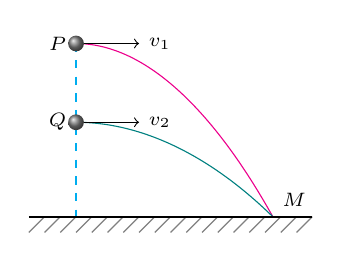
\begin{tikzpicture}[font=\scriptsize]
	\draw[dashed,cyan] (0,2.2)--(0,0);
	\draw[magenta] (0,2.2)coordinate(P) parabola bend (0,2.2) (2.5,0);
	\draw[teal] (0,1.2)coordinate(Q) parabola bend (0,1.2) (2.5,0);
	\foreach \c/\v in {P/v_1,Q/v_2}{
		\draw[->] (\c)--++(.8,0)node[right]{ \(\v\)};
		\shade[ball color=gray] (\c)node[left]{ \(\c\)} circle(.1);}
	\foreach \x in {-.6,-.4,...,3}
		\draw[gray] (\x,-.2)--++(.2,.2);
	\draw[thick] (-.6,0)--(3,0);
	\node at(2.5,0)[above right]{ \(M\)};
\end{tikzpicture}
\begin{choices}
	\item 一定是\(P\)先抛出的，并且\(v_1 = v_2\)
	\item 一定是\(P\)先抛出的，并且\(v_1 < v_2\)
	\item 一定是\(Q\)先抛出的，并且\(v_1 = v_2\)
	\item 一定是\(Q\)先抛出的，并且\(v_1 > v_2\)
\end{choices}
\begin{answer}
	B\qquad 提示：
\end{answer}